% ---------------------------------------------------------------------
% Defesa de TCC — Aquário
% Compilar:  tectonic -X compile slides.tex --outdir build
% As figuras vêm de ../figuras/, as mesmas da monografia.
% ---------------------------------------------------------------------
\documentclass[aspectratio=169,11pt]{beamer}

\usepackage[utf8]{inputenc}
\usepackage[T1]{fontenc}
\usepackage[brazil]{babel}
\usepackage{booktabs}
\usepackage{graphicx}
\graphicspath{{../figuras/}{../config/}}

% ---- visual enxuto, sem barras nem enfeites -------------------------
\usetheme{default}
\usecolortheme{default}
\setbeamertemplate{navigation symbols}{}
\setbeamertemplate{itemize items}[circle]
\setbeamercolor{structure}{fg=azul}
\setbeamerfont{frametitle}{size=\large,series=\bfseries}
\setbeamertemplate{frametitle}{%
  \vspace{0.7em}\hspace{0.2em}\insertframetitle\par\vspace{-0.4em}}
\setbeamertemplate{footline}{%
  \hfill\scriptsize\color{gray!70}\insertframenumber\hspace{1.2em}\vspace{0.6em}}

\definecolor{azul}{HTML}{1F5FBF}
\definecolor{cinza}{HTML}{4A5A6A}
\newcommand{\destaque}[1]{{\color{azul}\textbf{#1}}}
\newcommand{\nota}[1]{{\footnotesize\color{cinza}#1}}

% número grande com legenda embaixo
\newcommand{\bignum}[2]{%
  \begin{minipage}[t]{0.23\textwidth}\centering
  {\color{azul}\fontsize{30}{34}\selectfont\textbf{#1}}\\[0.3em]
  \nota{#2}\end{minipage}}

\title{Aquário}
\subtitle{Projeto e desenvolvimento de um hub acadêmico\\open-source para o CI/UFPB}
\author{Tiago Trindade de Oliveira}
\institute{Orientador: Prof.\ Dr.\ Moisés Dantas dos Santos}
\date{7 de agosto de 2026}

\begin{document}

% ---------------------------------------------------------------------
\begin{frame}[plain]
  \vspace{1.2em}
  \centering\includegraphics[height=1.5cm]{logo-ufpb.png}\\[1.4em]
  {\Huge\bfseries\color{azul}Aquário}\\[0.7em]
  {\large Um hub acadêmico open-source para o CI/UFPB}\\[2.2em]
  {\normalsize Tiago Trindade de Oliveira}\\[0.4em]
  \nota{Orientador: Prof.\ Dr.\ Moisés Dantas dos Santos}\\[1.6em]
  \nota{Centro de Informática \textperiodcentered{} UFPB \textperiodcentered{} 7 de agosto de 2026}
\end{frame}

% ======================= PROBLEMA ====================================
\begin{frame}{O problema}
  \vspace{0.5em}
  O CI tem um ecossistema rico --- laboratórios, grupos, ligas, projetos,
  oportunidades.\\[0.9em]

  \pause
  Mas o acesso a ele é \destaque{fragmentado e dependente do acaso}:
  \begin{itemize}
    \item apresentações na Semana da Computação
    \item convites informais no corredor
    \item perguntas em grupos de WhatsApp
  \end{itemize}
  \vspace{0.9em}

  \pause
  Ferramentas úteis existem --- SACI, mapas, calendário --- mas \destaque{isoladas},
  sem integração entre si.
  \vspace{0.9em}

  \pause
  \nota{O período inicial é crítico: desconhecimento do ambiente institucional está
  entre os fatores associados à evasão nos primeiros semestres (VELOZO \textit{et al.}, 2025).}
\end{frame}

\begin{frame}{Quem perde com isso}
  \vspace{1.2em}
  \begin{columns}[T]
    \column{0.31\textwidth}
      \destaque{Ingressantes}\\[0.4em]
      \nota{Chegam sem referências e descobrem tarde o que existe.}
    \column{0.31\textwidth}
      \destaque{Veteranos}\\[0.4em]
      \nota{Desconhecem parte do que o próprio centro oferece.}
    \column{0.31\textwidth}
      \destaque{O próprio centro}\\[0.4em]
      \nota{Sem base viva e pública, não consegue apresentar nem manter memória do que produz.}
  \end{columns}
  \vspace{2em}
  \pause
  \centering\nota{Nenhum portal nacional inspecionado reunia o escopo
  necessário --- sete universidades consultadas.}
\end{frame}

% ======================= TRABALHOS RELACIONADOS ======================
\begin{frame}{O que já existe}
  \vspace{0.6em}
  \begin{itemize}\setlength\itemsep{0.5em}
    \item \destaque{Sistemas de gestão acadêmica} (SIGAA e afins) --- orientados
      a processos institucionais: matrícula, histórico, frequência.\\
      \nota{Função operacional; não se propõem a dar visibilidade ao que o centro produz.}
    \item \destaque{Páginas institucionais} --- sete cursos de computação
      consultados, em quatro regiões.\\
      \nota{Cinco publicam listagens estáticas; em duas (UFRJ e UFRN) não há listagem
      de laboratórios. Nenhuma tem busca, filtro ou descrição de projetos.}
    \item \destaque{City Tech OpenLab} (CUNY) --- o mais próximo internacionalmente,
      mas focado em pedagogia aberta.
    \item \destaque{SIAC} (UNIFESSPA) --- o mais próximo no Brasil: sem dados de
      adoção, organizado por \textit{chatbot}, e não é código aberto comunitário.
  \end{itemize}
  \vspace{0.6em}
  \pause
  \centering\nota{Inspeção por conveniência, não revisão sistemática ---
  delimita o panorama consultado.}
\end{frame}

\begin{frame}{Onde o Aquário se posiciona}
  \vspace{0.8em}
  \centering\small
  \begin{tabular}{lcccc}
    \toprule
    & \textbf{Aquário} & \shortstack{\textbf{Páginas}\\\textbf{instituc.}}
    & \shortstack{\textbf{City Tech}\\\textbf{OpenLab}} & \textbf{SIGAA} \\
    \midrule
    Busca e filtragem do ecossistema      & Sim & Não & Parcial & Não \\
    Descrição detalhada de projetos       & Sim & Não & Sim     & Parcial \\
    Ferramentas acadêmicas integradas     & Sim & Não & Não     & Sim \\
    Acesso público sem autenticação       & Sim & Sim & Parcial & Não \\
    Código aberto e replicável            & Sim & Não & Parcial & Não \\
    Mantido pela comunidade discente      & Sim & Não & Não     & Não \\
    \bottomrule
  \end{tabular}
  \vspace{1.2em}

  \pause
  \begin{minipage}{0.84\textwidth}\centering
  Um espaço pouco explorado: plataforma \destaque{interativa} e
  \destaque{mantida pela própria comunidade}, voltada a tornar visível
  o que o centro tem a oferecer.
  \end{minipage}
\end{frame}

\begin{frame}{Objetivo}
  \vspace{1.6em}
  \begin{center}
  \large
  Projetar, desenvolver, \destaque{disponibilizar em produção}\\
  e \destaque{avaliar a adoção} de uma plataforma web open-source\\
  de centralização e divulgação das informações do CI/UFPB.
  \end{center}
  \vspace{1.8em}
  \pause
  \centering\nota{Ênfase nas duas últimas: não é protótipo, e a adoção é medida.}
\end{frame}

% ======================= O SISTEMA ===================================
\begin{frame}[plain]
  \centering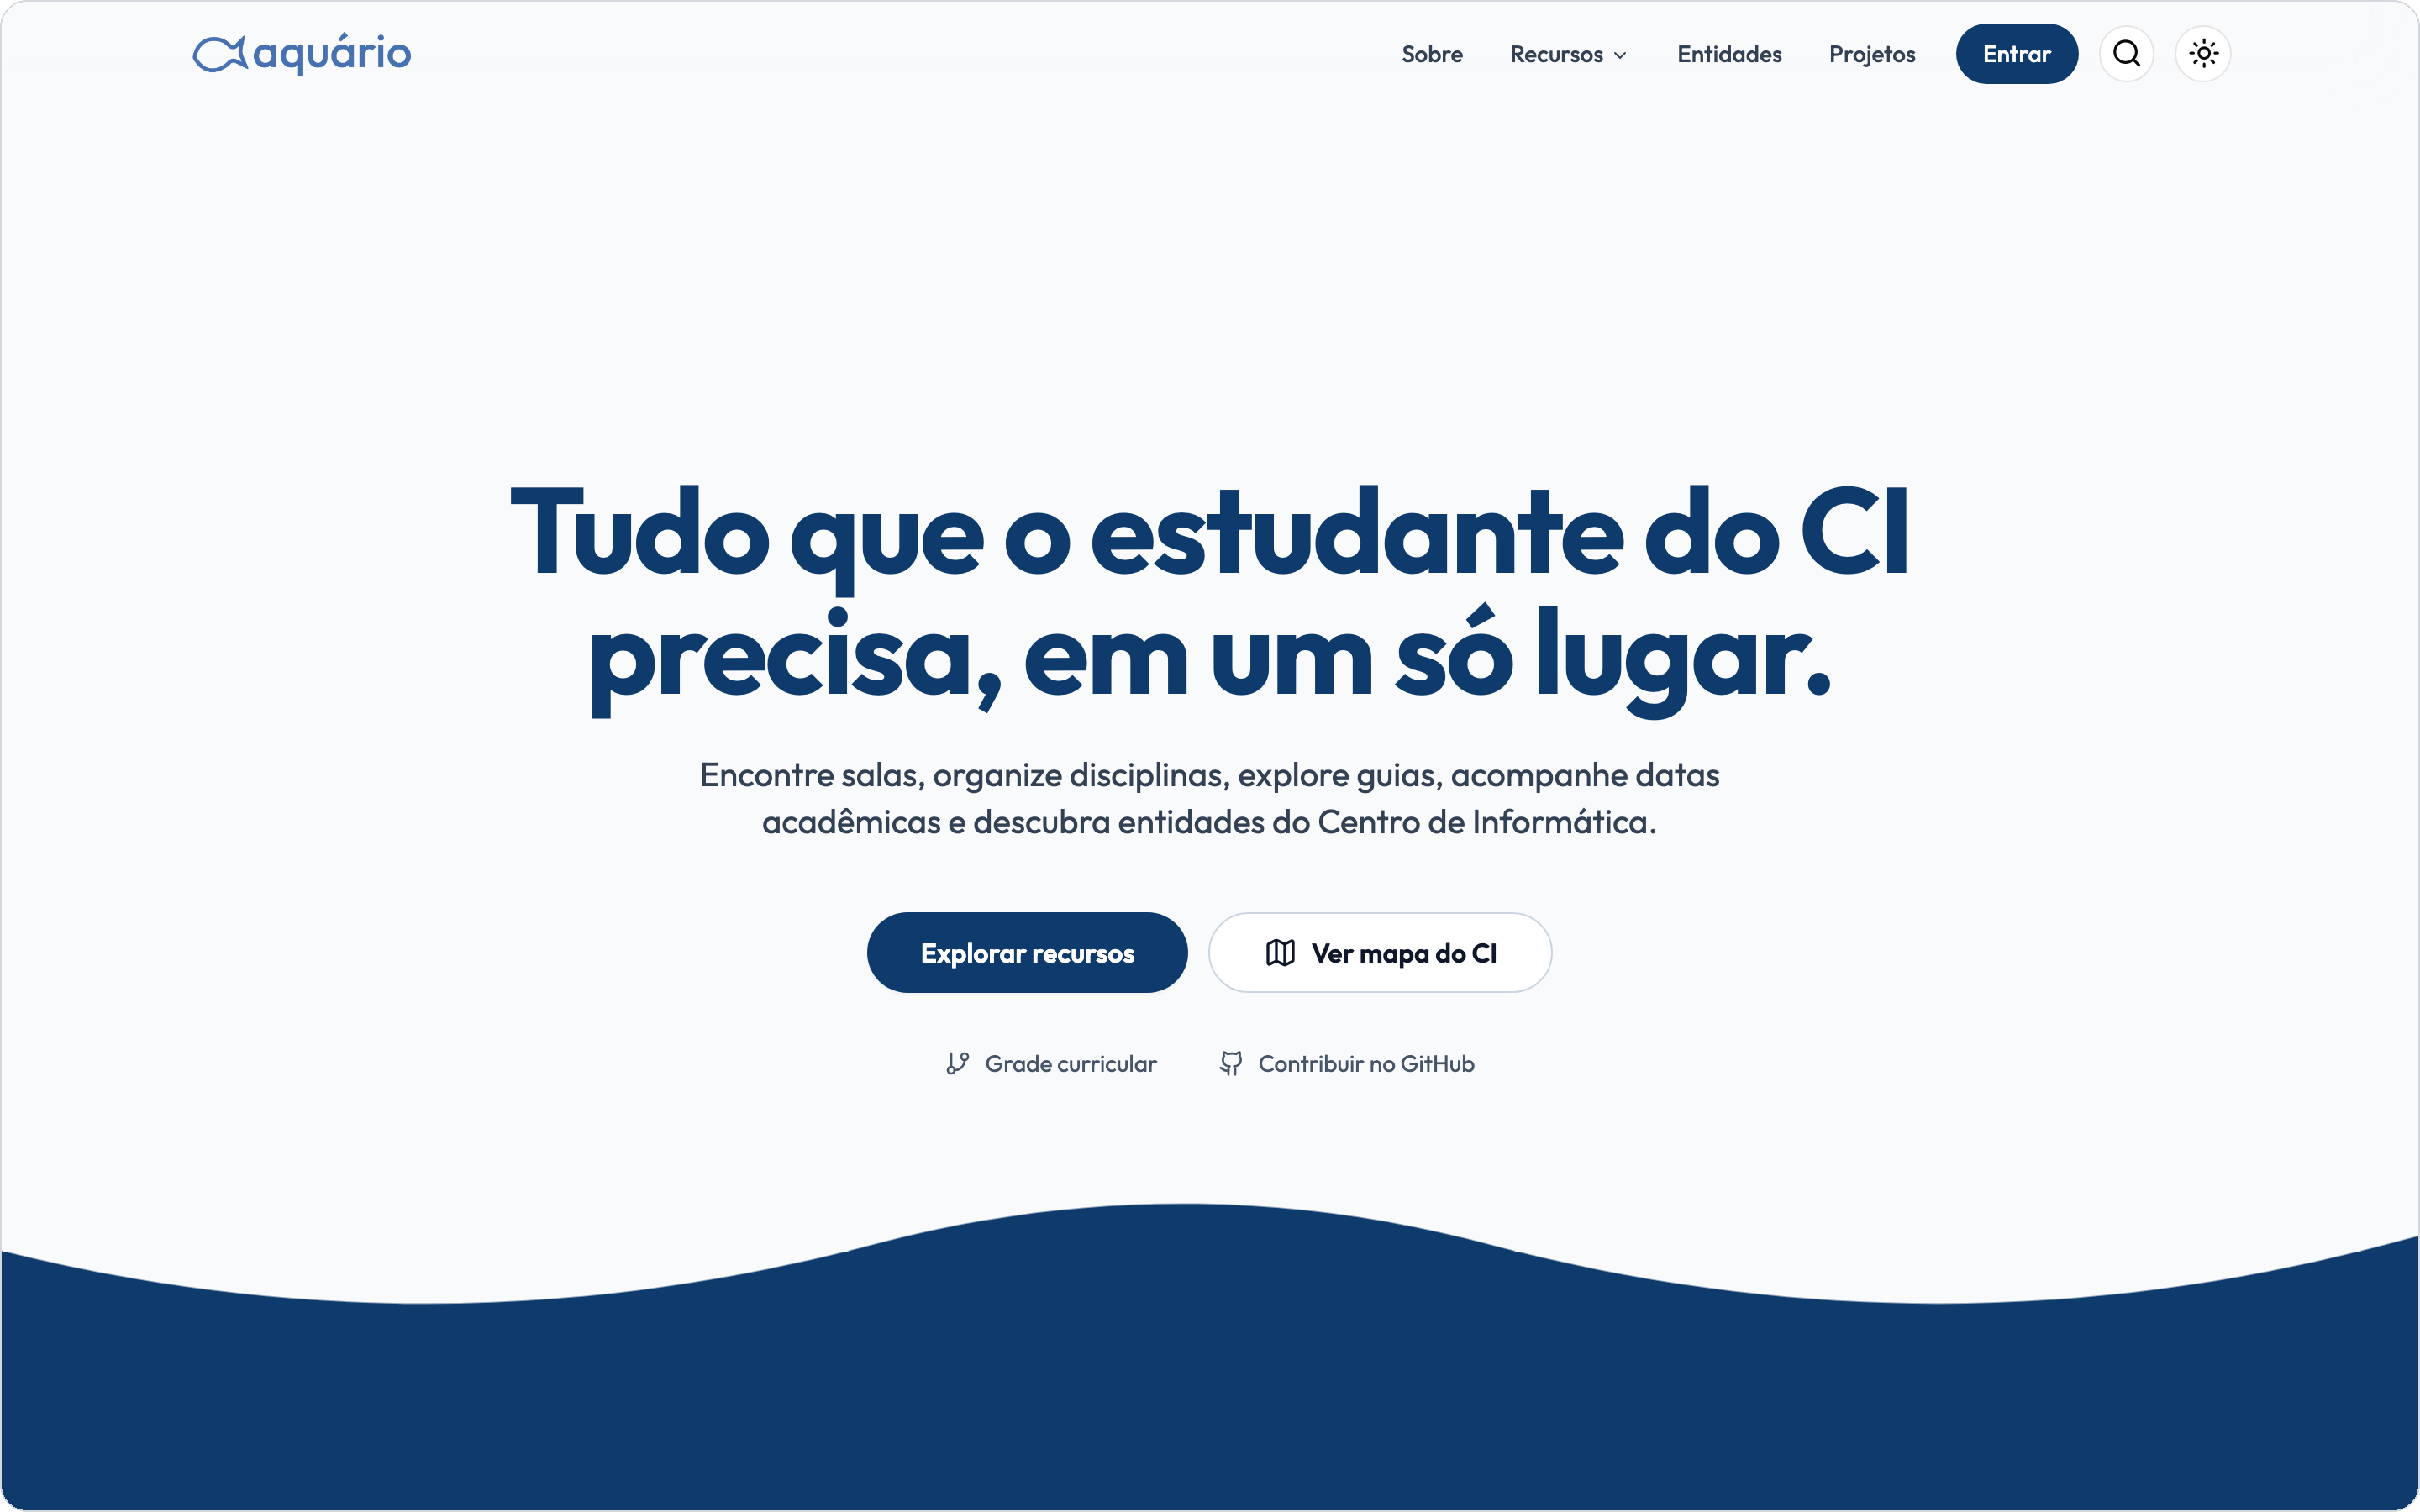
\includegraphics[width=0.92\textwidth]{landing-page.png}\\[0.4em]
  \nota{aquarioufpb.com --- no ar desde novembro de 2025}
\end{frame}

\begin{frame}{Dez módulos em produção}
  \vspace{0.6em}
  \begin{columns}[T]
    \column{0.48\textwidth}
      \begin{itemize}\setlength\itemsep{0.35em}
        \item Diretório de entidades
        \item Projetos acadêmicos
        \item Guias curriculares
        \item Grades curriculares interativas
        \item Minhas Disciplinas
      \end{itemize}
    \column{0.48\textwidth}
      \begin{itemize}\setlength\itemsep{0.35em}
        \item Calendário acadêmico
        \item Mapas dos prédios
        \item Busca global
        \item Perfil público de usuário
        \item Painel administrativo
      \end{itemize}
  \end{columns}
  \vspace{1.2em}
  \pause
  \centering\nota{Onze requisitos funcionais especificados, todos verificados por
  execução em produção.}
\end{frame}

\begin{frame}[plain]
  \centering
  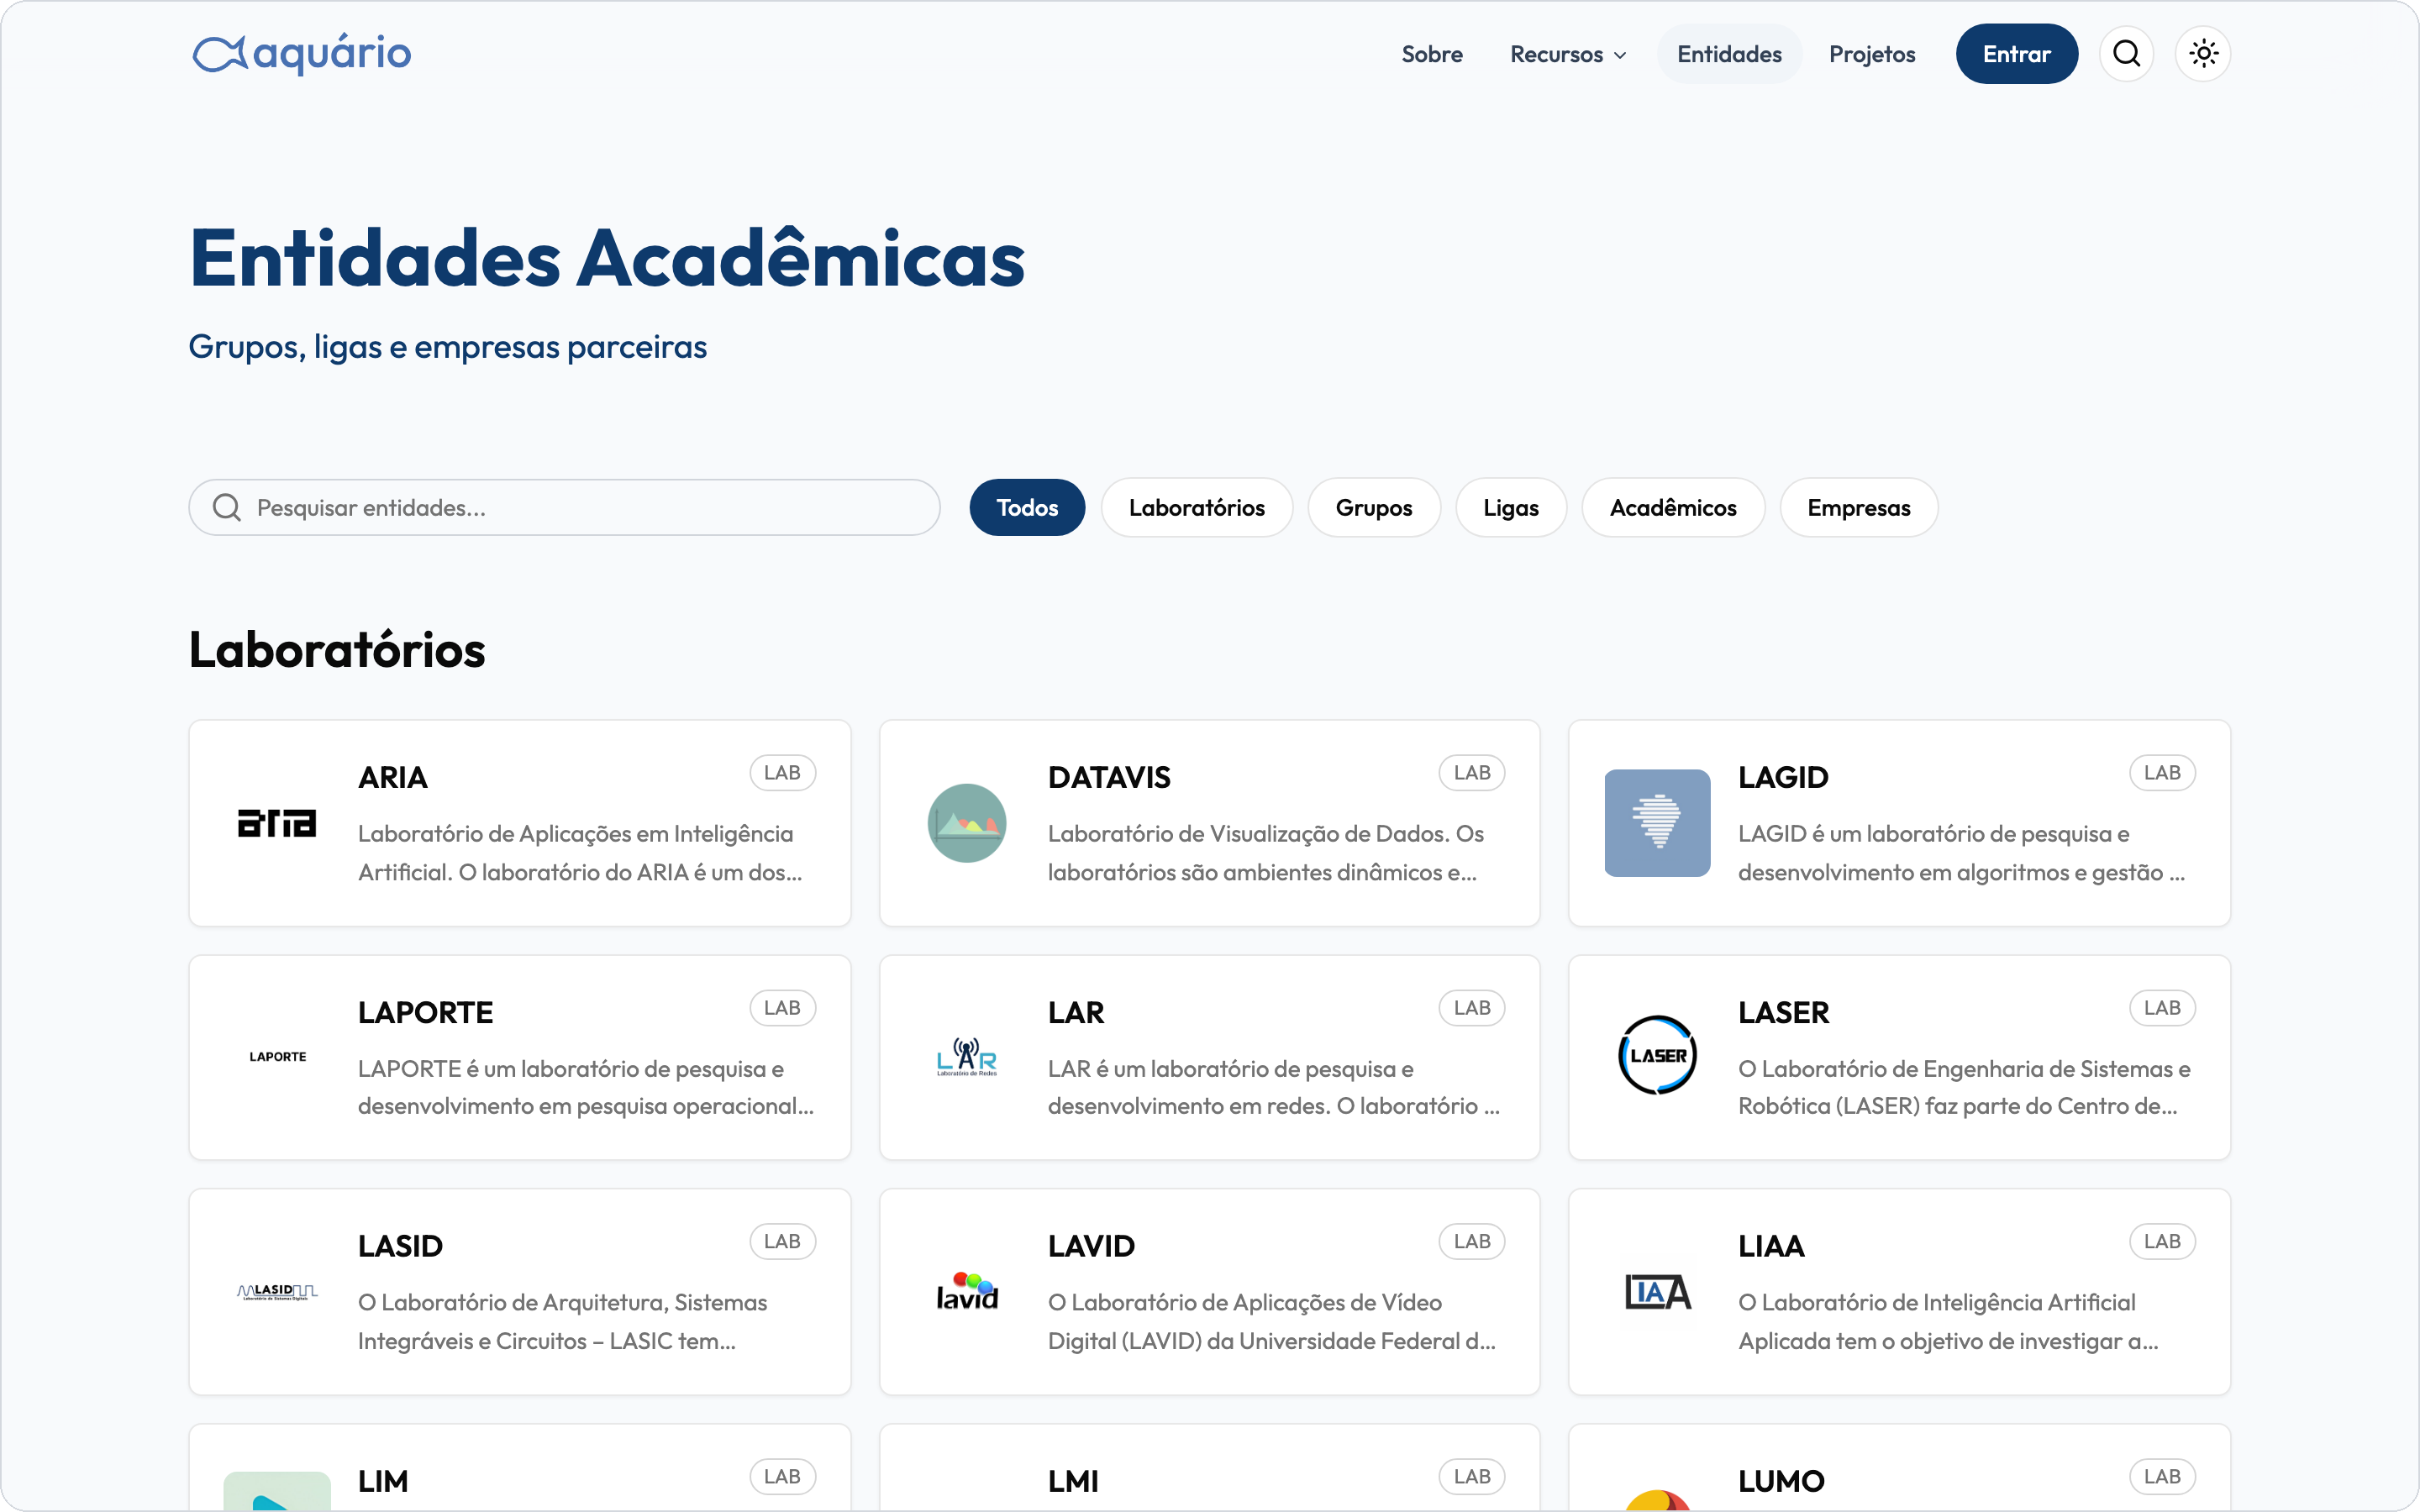
\includegraphics[height=0.44\textheight]{diretorio-entidades.png}\hspace{0.4em}
  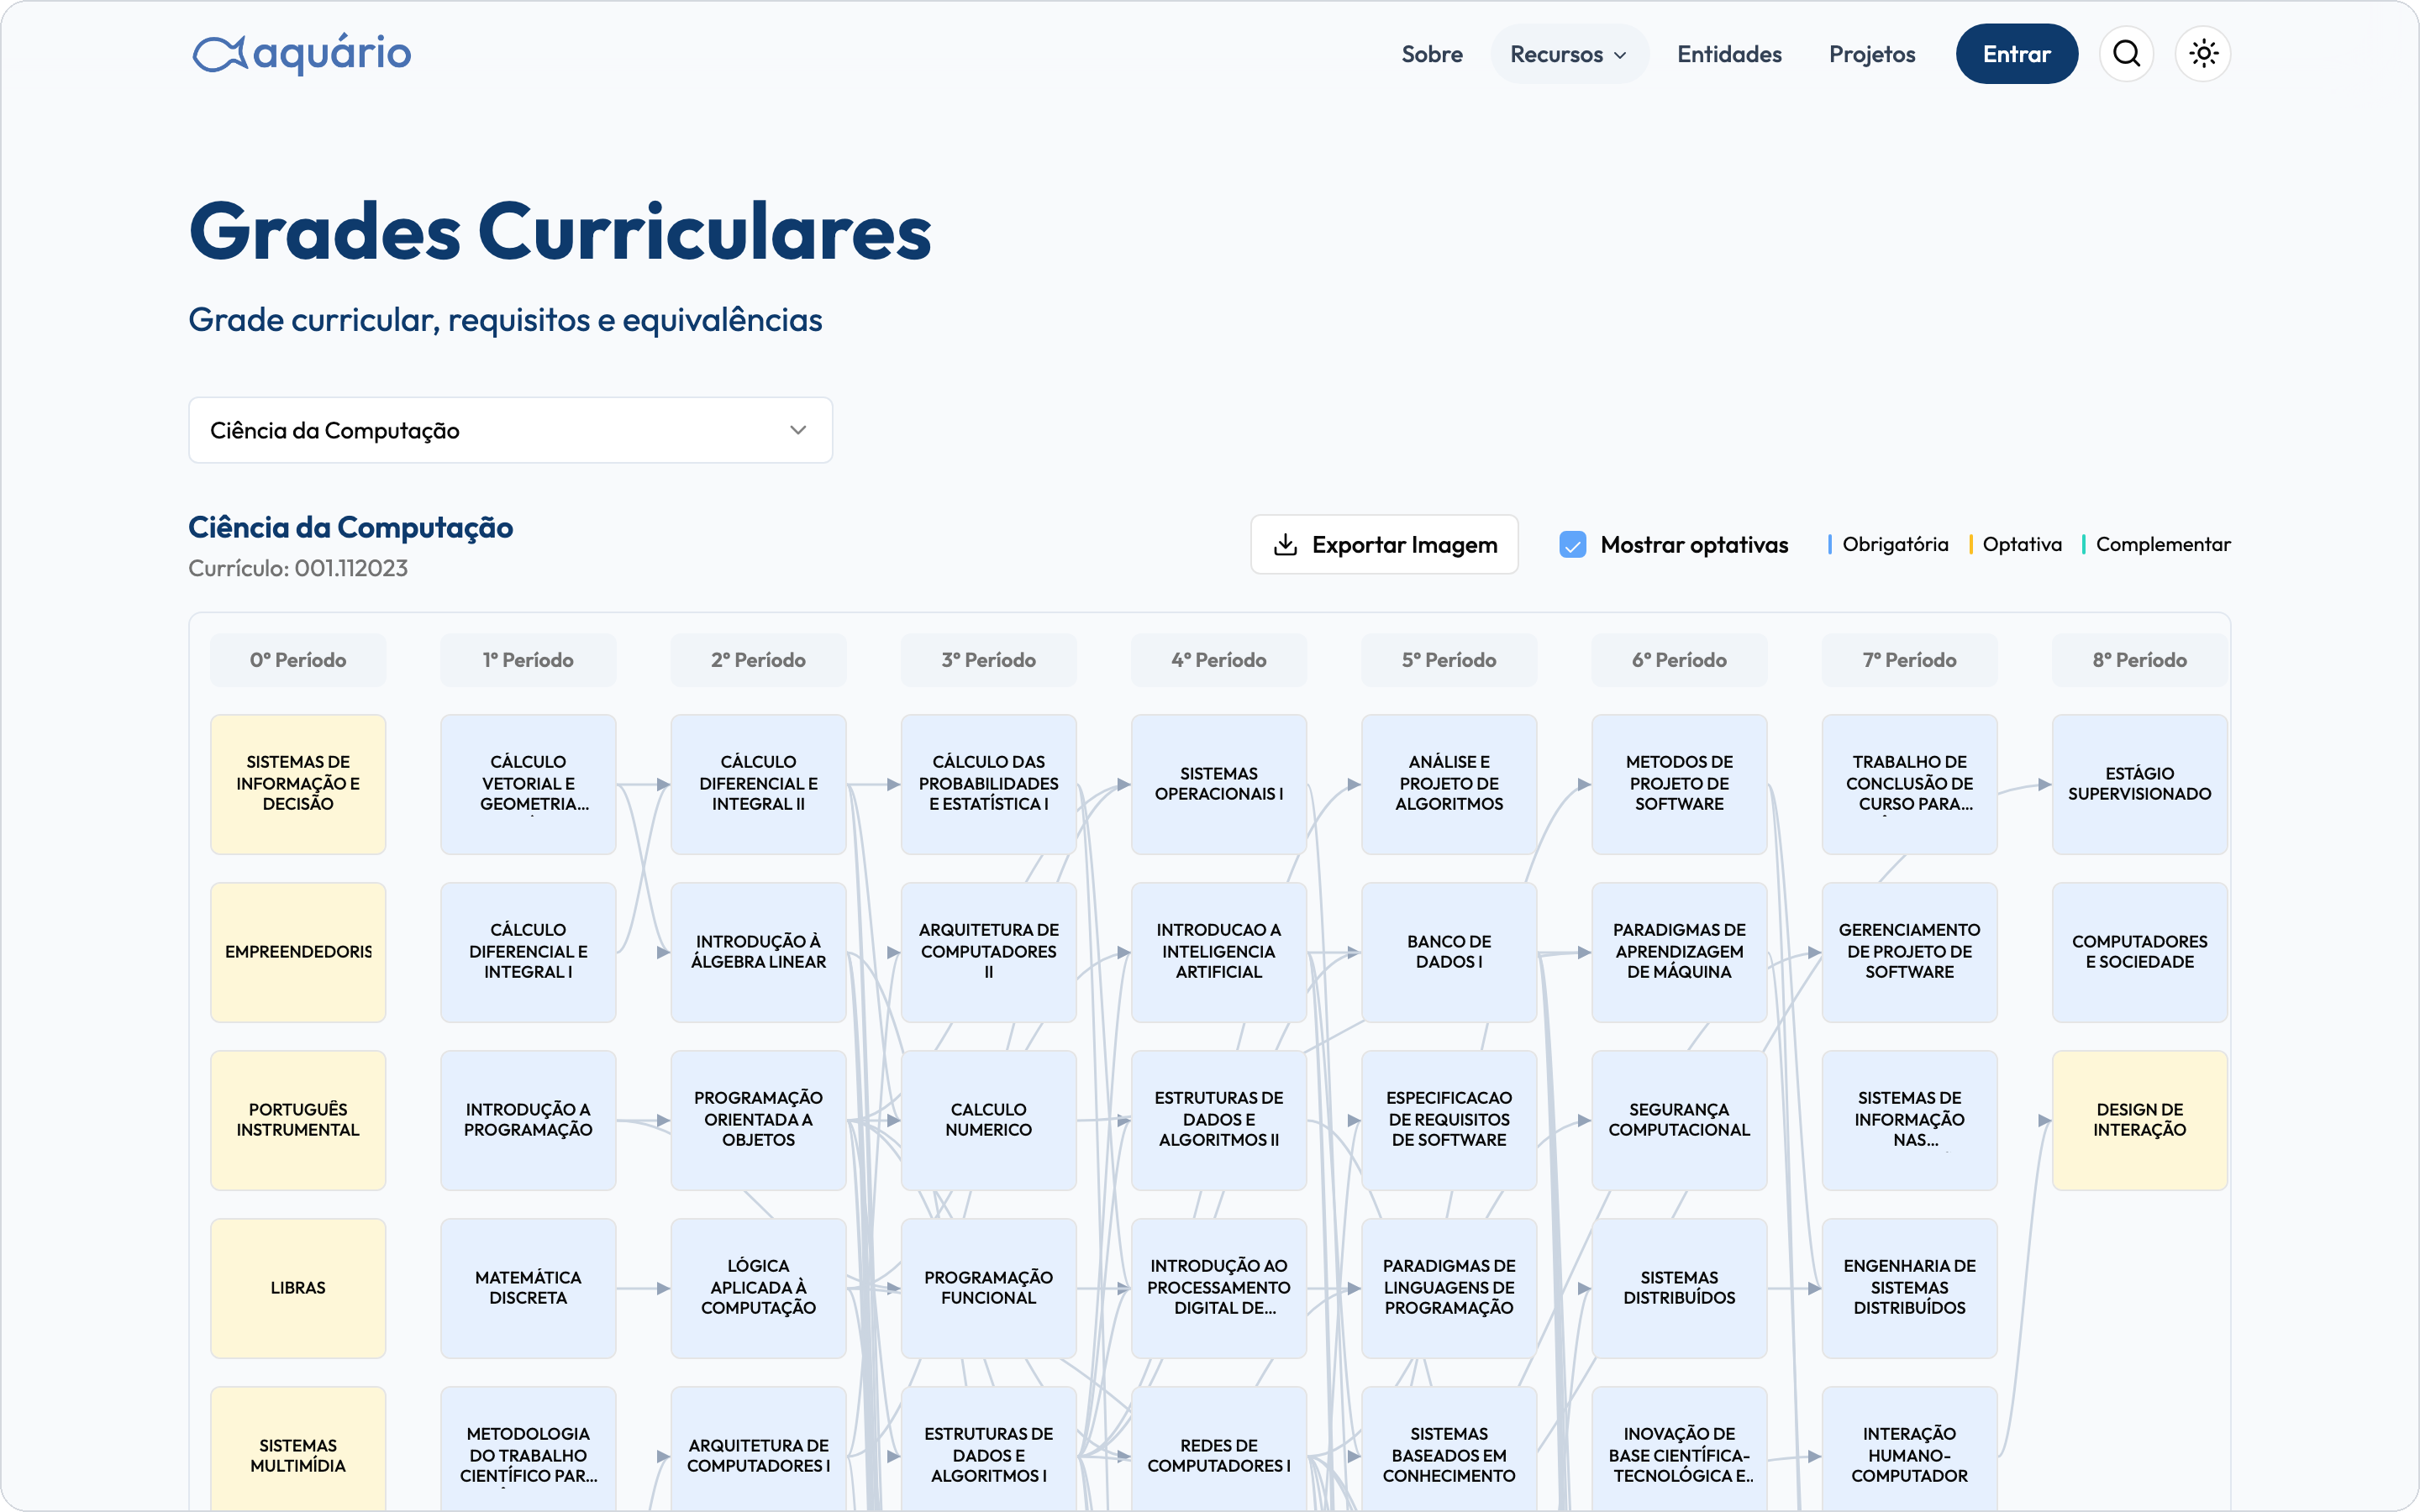
\includegraphics[height=0.44\textheight]{grades-curriculares.png}\\[0.5em]
  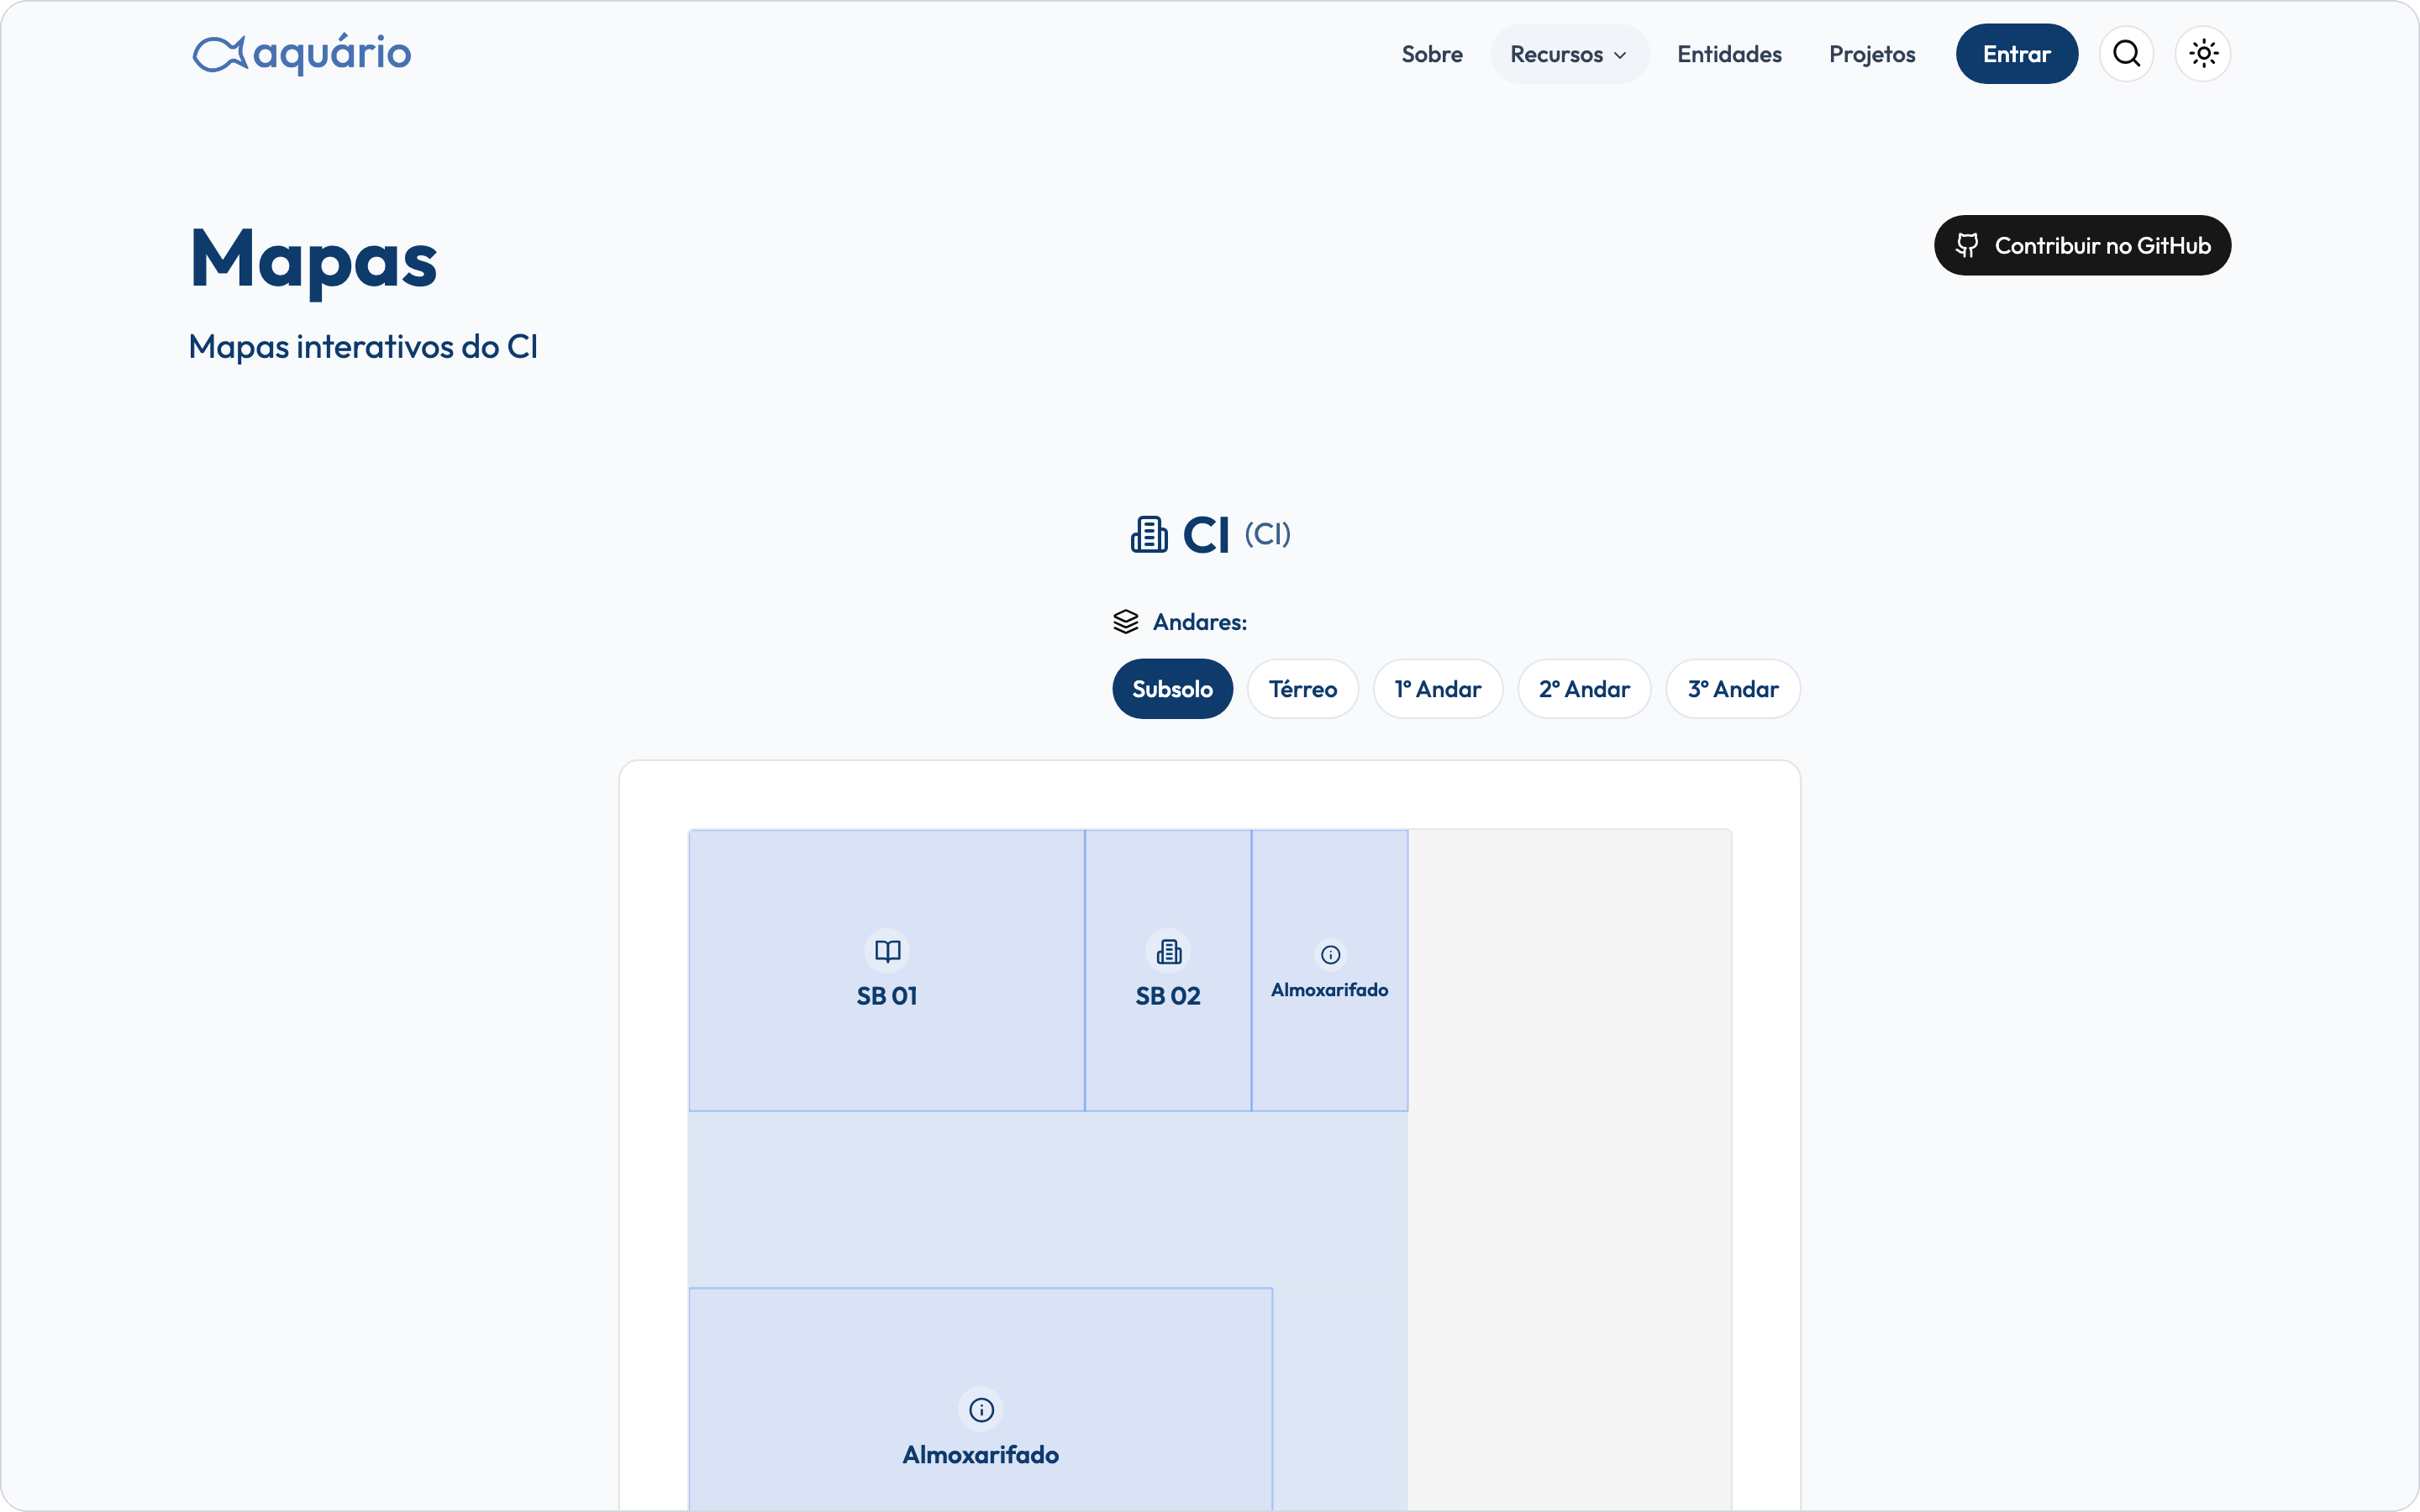
\includegraphics[height=0.44\textheight]{mapas.png}\hspace{0.4em}
  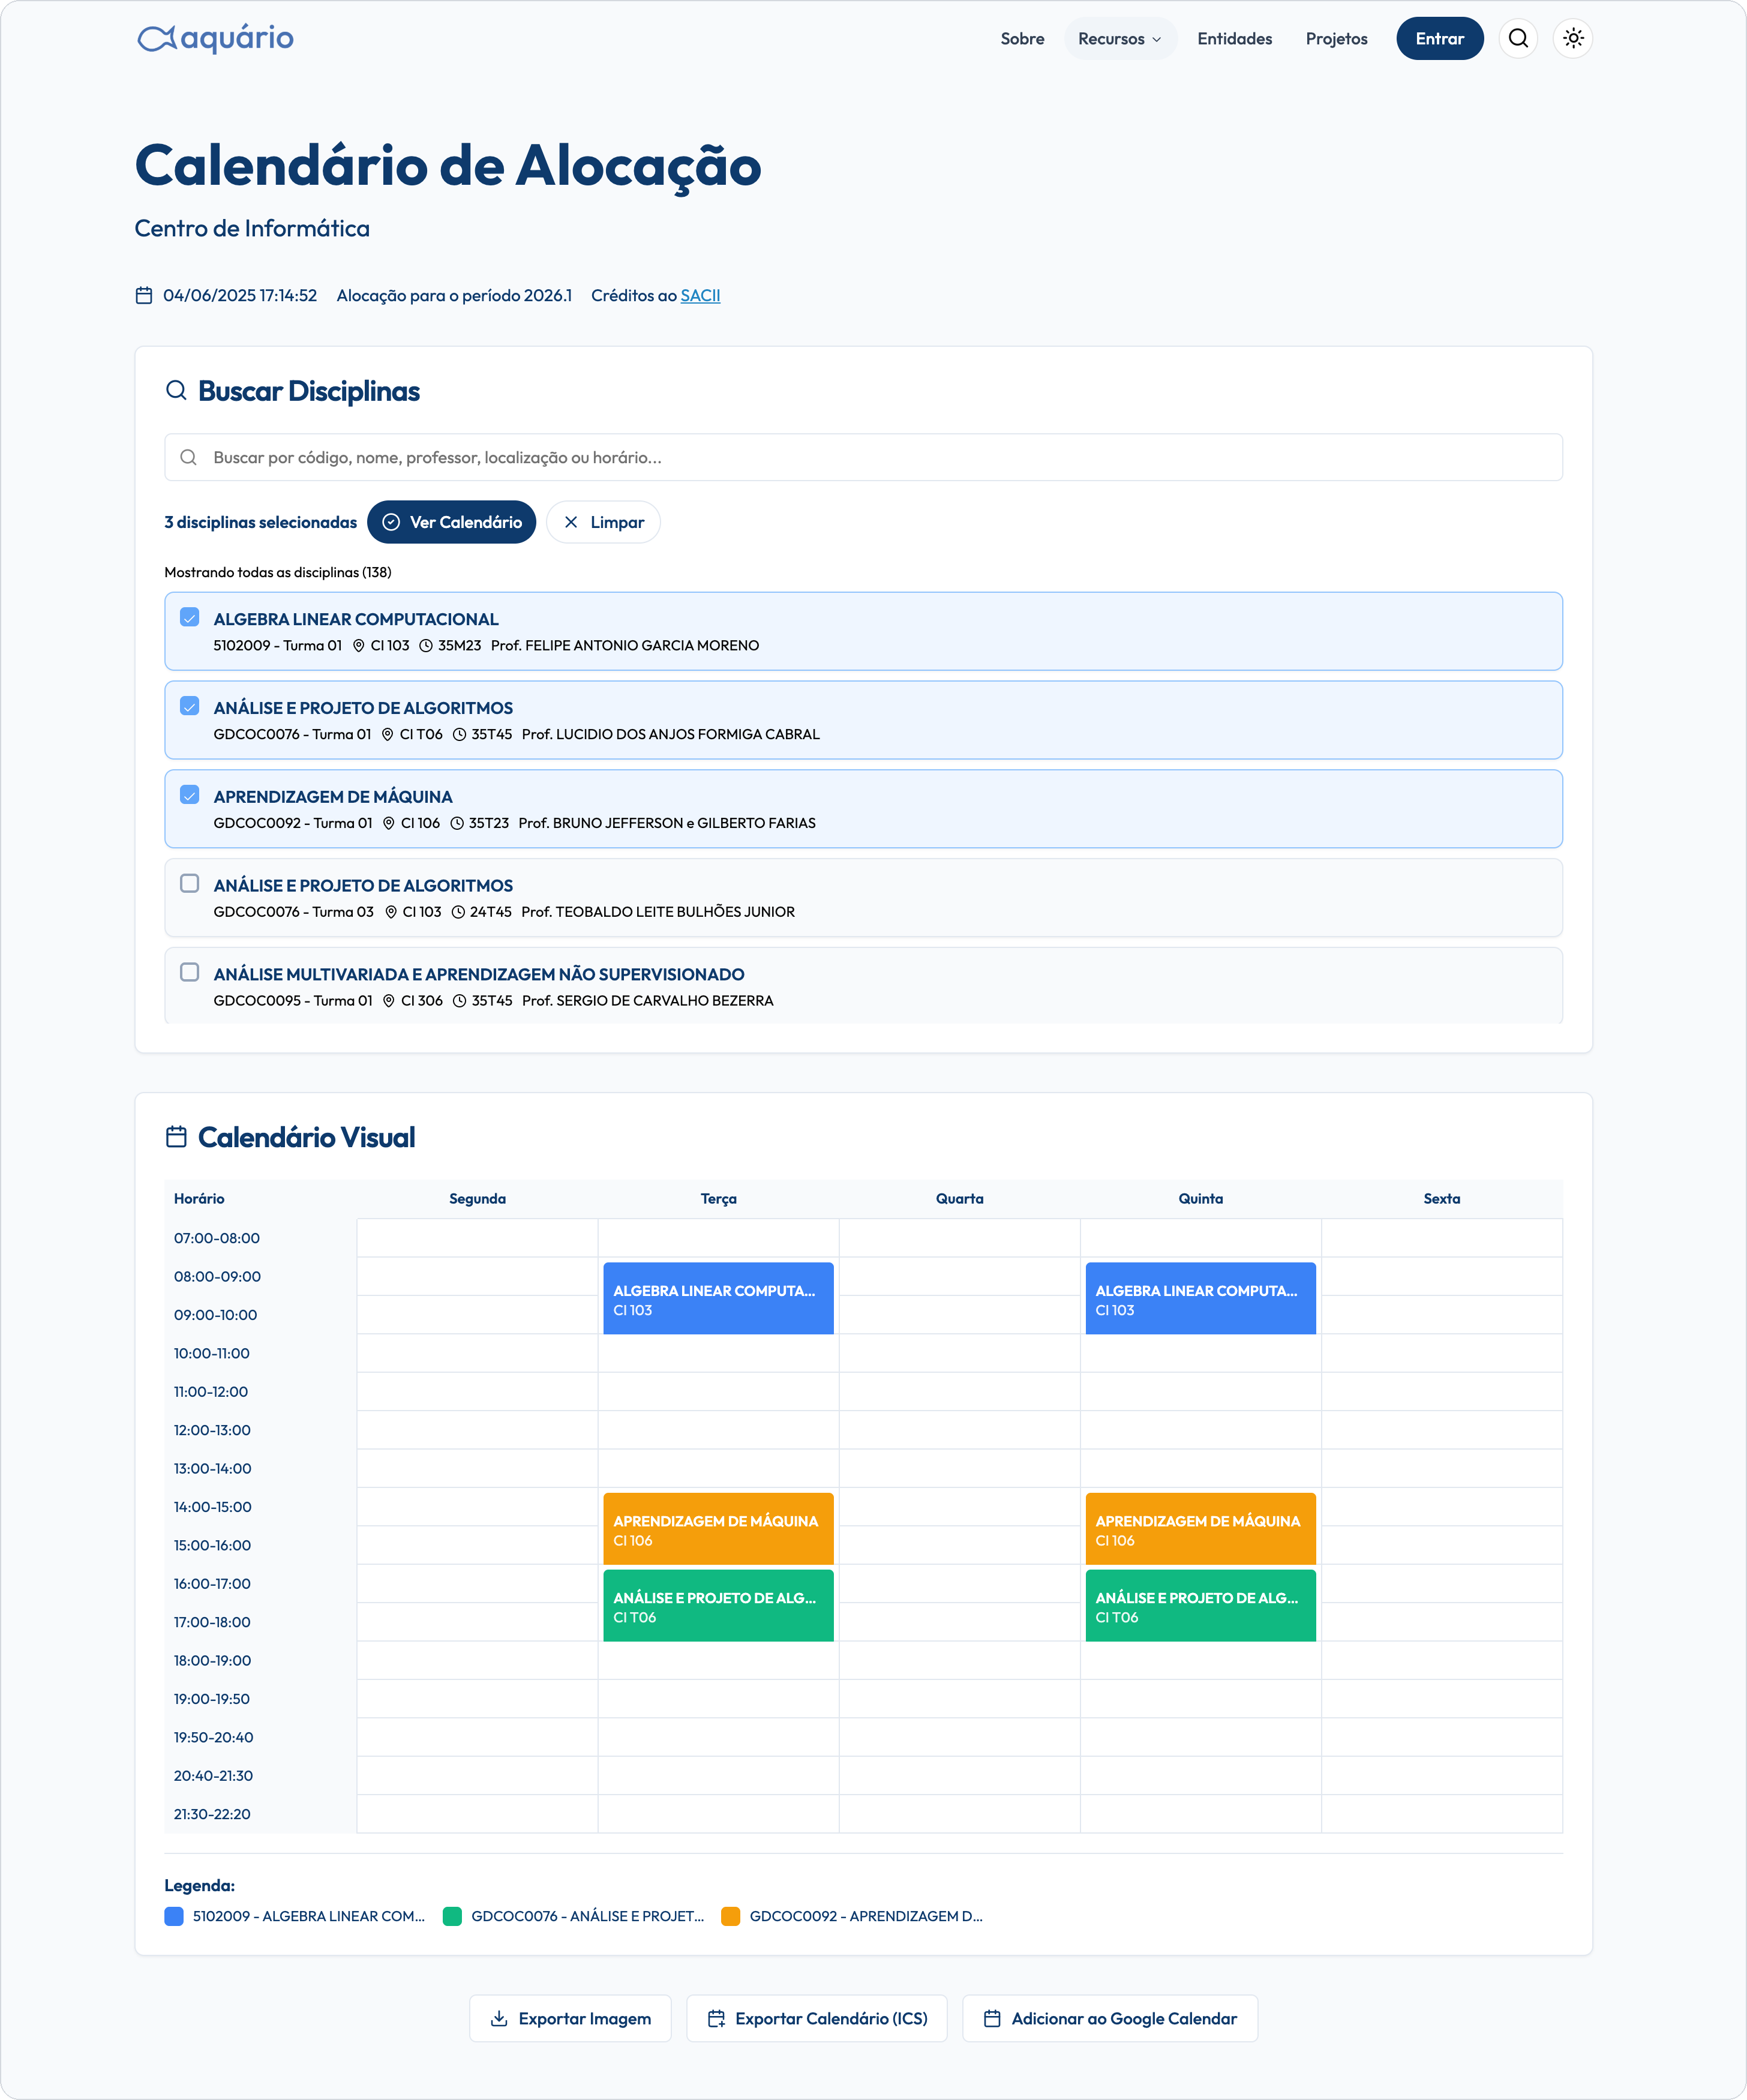
\includegraphics[height=0.44\textheight]{minhas-disciplinas.png}
\end{frame}

% ======================= DECISÕES ====================================
\begin{frame}{A decisão que orientou todas as outras}
  \vspace{0.5em}
  O ponto de partida não é técnico, é \destaque{organizacional}:
  \vspace{0.5em}
  \begin{quote}\itshape\color{cinza}
  a plataforma precisa ser mantida por uma equipe distribuída,\\
  rotativa e voluntária --- e sem orçamento.\\[0.3em]
  Quem escreveu cada parte não estará lá quando ela mudar.
  \end{quote}
  \vspace{0.8em}
  \pause
  Disso derivam cinco critérios:
  \begin{enumerate}\setlength\itemsep{0.25em}
    \item repositório único para \textit{frontend} e \textit{backend}
    \item bibliotecas de componentes prontas
    \item popularidade da tecnologia
    \item tipagem estática
    \item implantação simples e sem custo
  \end{enumerate}
  \vspace{0.7em}
  \pause
  \centering\nota{Convergem no Next.js + Vercel. Custo de infraestrutura: zero,
  exceto o domínio.}
\end{frame}

\begin{frame}[plain]
  \centering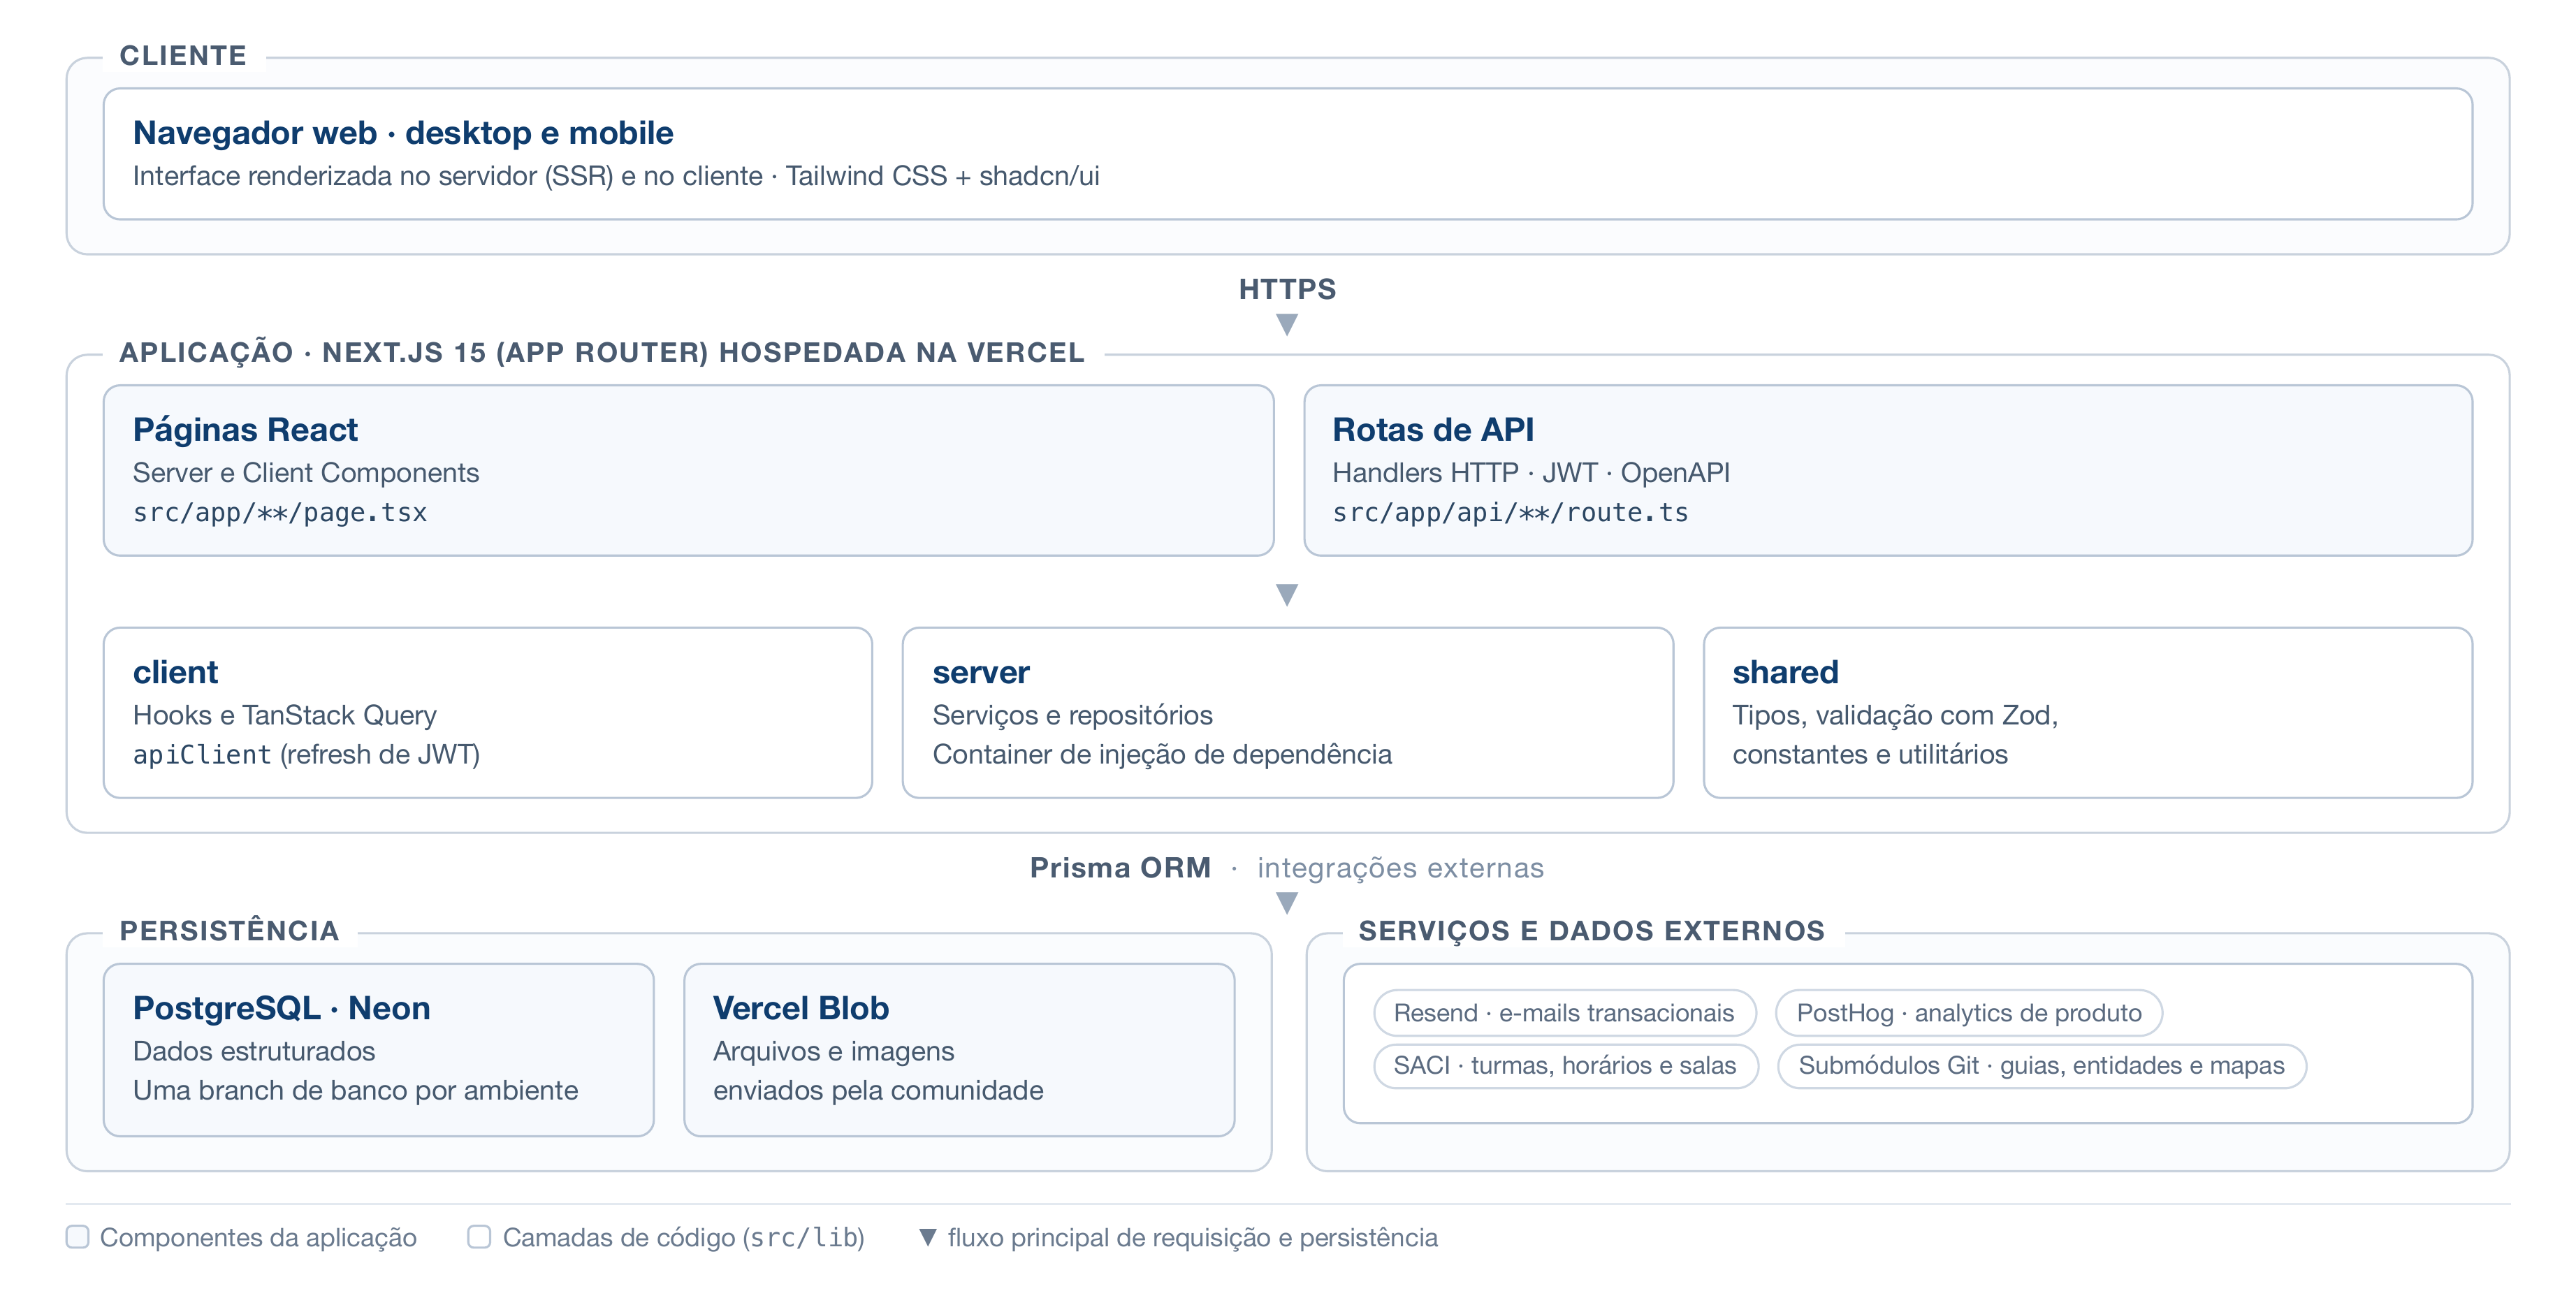
\includegraphics[width=0.86\textwidth]{arquitetura-sistema.pdf}
\end{frame}

\begin{frame}[plain]
  \centering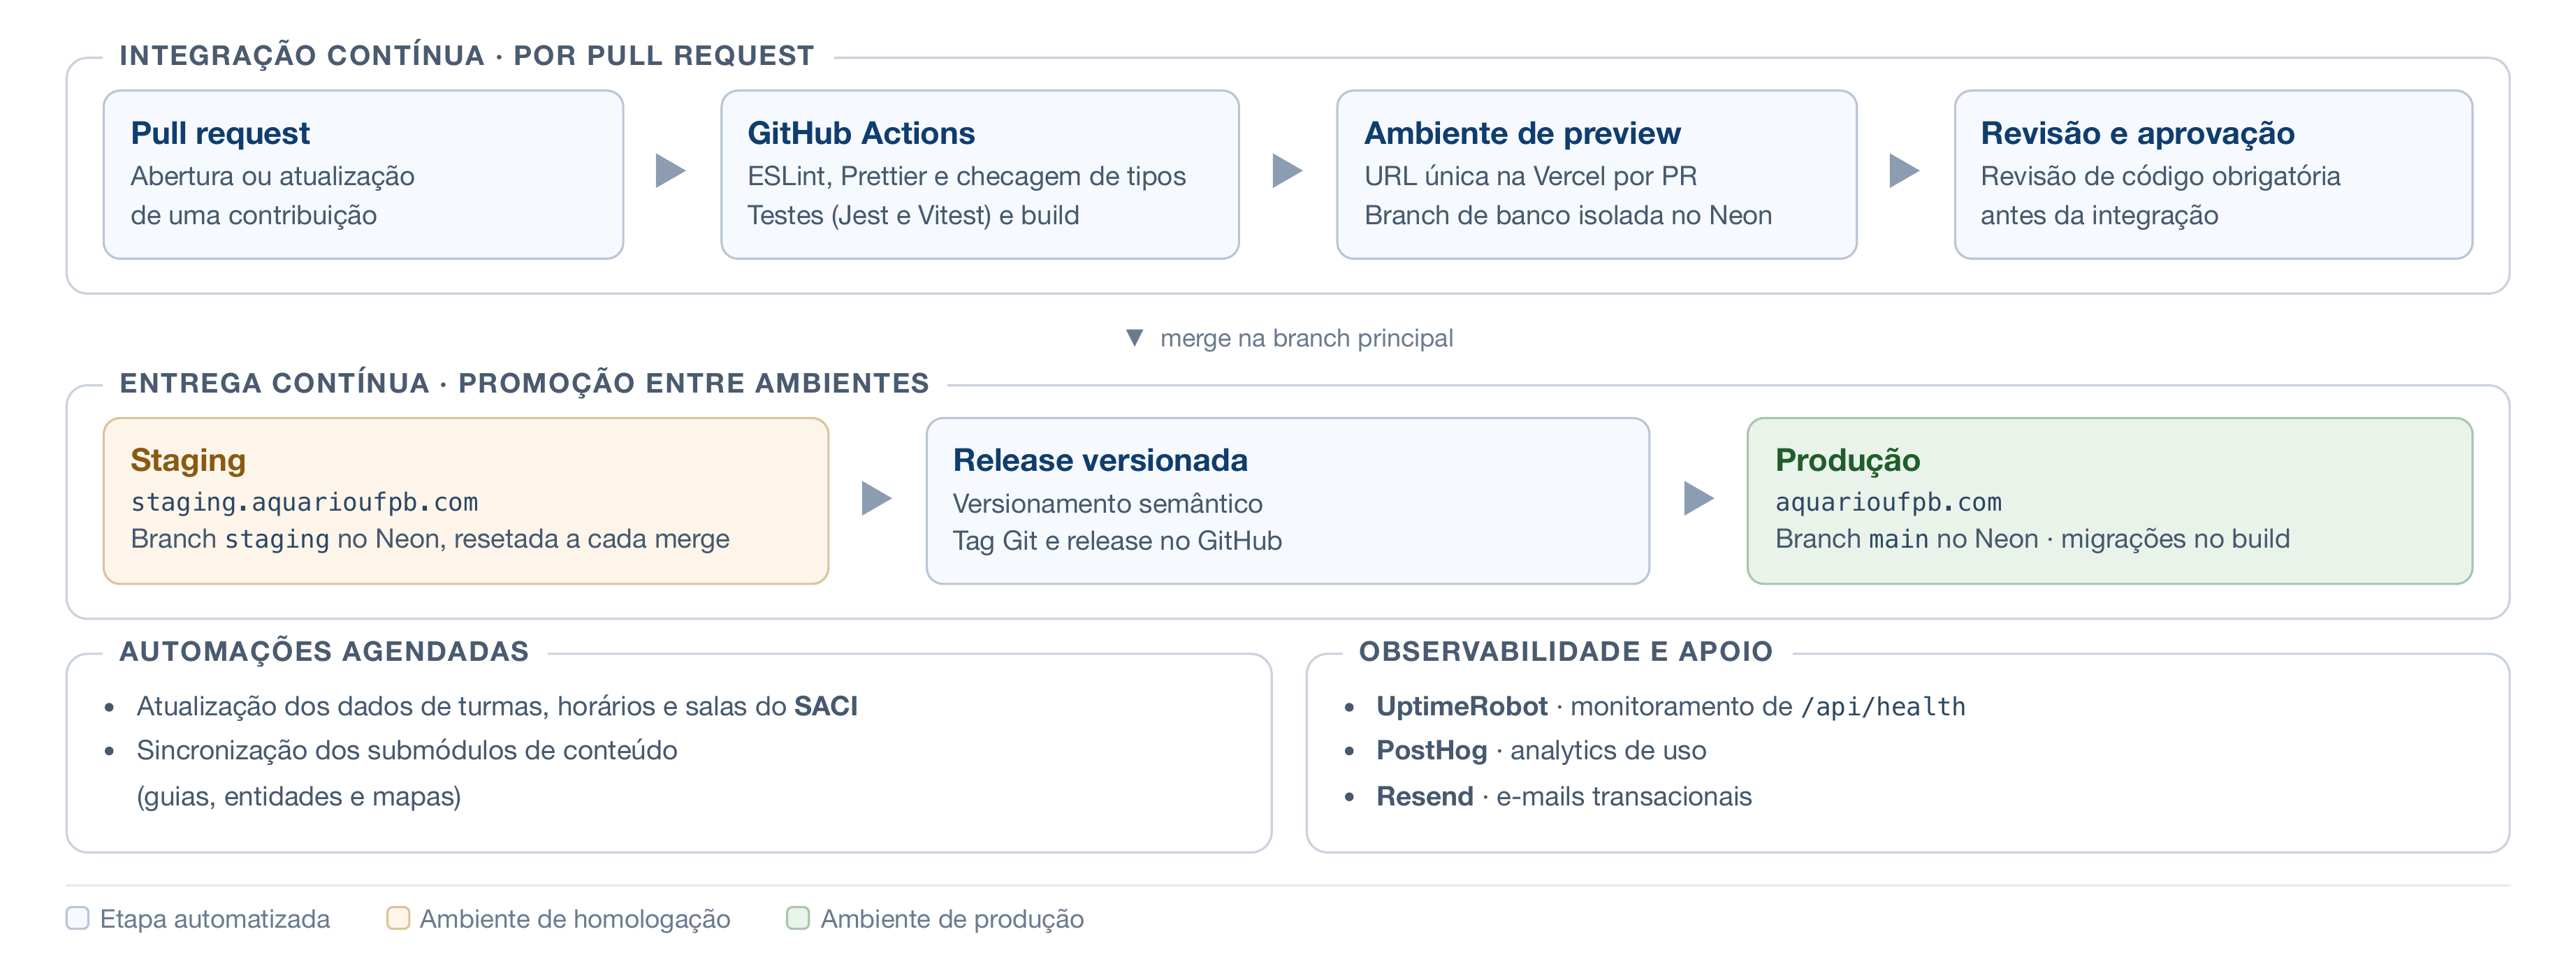
\includegraphics[width=0.94\textwidth]{infraestrutura-cicd.pdf}\\[0.3em]
  \nota{Quatro ambientes \textperiodcentered{} banco isolado por \textit{pull request} \textperiodcentered{} deploy a cada release}
\end{frame}

% ======================= MÉTODO ======================================
\begin{frame}{Natureza do trabalho}
  \vspace{0.7em}
  Relato de experiência de desenvolvimento de software, conduzido como
  \destaque{estudo de caso único} sobre a concepção, a implantação e a
  evolução inicial do Aquário.
  \vspace{1em}

  \pause
  \begin{columns}[T]
    \column{0.46\textwidth}
      \destaque{O que produz}\\[0.4em]
      \nota{Evidência sobre a viabilidade técnica e organizacional de uma
      solução em operação real, com dados de sete meses de uso.}
    \column{0.46\textwidth}
      \destaque{O que não permite}\\[0.4em]
      \nota{Generalização estatística e inferência causal. É um caso, num
      centro específico, observado por quem o construiu.}
  \end{columns}
  \vspace{1.2em}

  \pause
  \centering\nota{Duas delimitações assumidas: o problema não foi precedido de
  levantamento empírico junto aos estudantes, e o que se avalia é a adoção ---
  medida por uso efetivo --- e não a usabilidade.}
\end{frame}

\begin{frame}{O procedimento, em quatro etapas}
  \vspace{0.9em}
  \begin{enumerate}\setlength\itemsep{0.65em}
    \item \destaque{Caracterização do problema}\\
      \nota{Observação direta no centro, confrontada com a literatura sobre
      integração de ingressantes.}
    \item \destaque{Especificação}\\
      \nota{Onze requisitos funcionais e seis não funcionais, estes com
      \emph{metas verificáveis} --- não apenas declaradas.}
    \item \destaque{Implementação}\\
      \nota{Iterativa, com entrega contínua em produção e revisão obrigatória
      por pares a cada mudança. 27 releases no período.}
    \item \destaque{Aferição da adoção}\\
      \nota{Recorte temporal fechado e três fontes independentes de dados.}
  \end{enumerate}
\end{frame}

\begin{frame}{Como a adoção foi medida}
  \vspace{0.8em}
  Recorte fechado: \destaque{3 de novembro de 2025 a 9 de junho de 2026} --- 219 dias.\\
  \nota{Última release sob minha liderança: v1.8.0.}

  \vspace{1.2em}
  \pause
  Três fontes independentes:


  \vspace{0.5em}
  \begin{columns}[T]
    \column{0.31\textwidth}
      \destaque{Banco de produção}\\[0.3em]
      \nota{Ações persistidas. Não dependem de instrumentação nem sofrem com bloqueadores.}
    \column{0.31\textwidth}
      \destaque{Analytics}\\[0.3em]
      \nota{Navegação, inclusive de visitante anônimo. 37 eventos tipados.}
    \column{0.31\textwidth}
      \destaque{Repositório}\\[0.3em]
      \nota{Commits, contribuidores, releases.}
  \end{columns}
  \vspace{1.2em}
  \pause
  \centering\nota{Cada fonte compensa uma fraqueza da outra.}
\end{frame}

% ======================= RESULTADOS ==================================
\begin{frame}{O acervo deixou de ser uma estrutura vazia}
  \vspace{1.8em}
  \centering
  \bignum{157}{contas} \hfill
  \bignum{44}{entidades} \hfill
  \bignum{80}{projetos} \hfill
  \bignum{329}{disciplinas}
  \vspace{2.2em}

  \pause
  \nota{As 44 entidades cobrem laboratórios, grupos, ligas, empresas,
  centros acadêmicos e atlética --- e \destaque{todas} receberam ao menos um acesso
  no período.}
\end{frame}

\begin{frame}{O resultado que mais importa}
  \vspace{0.4em}
  \centering
  \begin{tabular}{lrr}
    \toprule
    \textbf{Funcionalidade} & \textbf{Usuários} & \textbf{Registros} \\
    \midrule
    Calendário de turmas do semestre   & 129 \; (82,2\%) & 956 \\
    Acompanhamento de grade curricular & 121 \; (77,1\%) & 2.423 \\
    Vínculo com ao menos uma entidade  & 93 \; (59,2\%)  & 239 \\
    \bottomrule
  \end{tabular}
  \vspace{1.4em}

  \pause
  \begin{minipage}{0.86\textwidth}
  A maioria não apenas visitou: \destaque{registrou dados pessoais} de progresso
  acadêmico e organização do semestre.
  \vspace{0.5em}

  \nota{Média de 20 disciplinas por estudante --- compatível com histórico completo,
  não com teste superficial. E são etapas que podiam ser puladas com um clique.}
  \end{minipage}
\end{frame}

\begin{frame}{Alcance}
  \vspace{1.4em}
  \centering
  \bignum{2.026}{sessões únicas} \hfill
  \bignum{6.976}{visualizações} \hfill
  \bignum{3,4}{páginas/sessão} \hfill
  \bignum{710}{pico semanal}
  \vspace{2em}

  \pause
  \nota{O pico coincide com o início do período letivo, em março.\\
  86,3\% dos acessos vêm do Brasil; João Pessoa é a cidade com maior volume.}
\end{frame}

\begin{frame}{O que não foi atendido}
  \vspace{0.6em}
  Seis requisitos não funcionais com metas verificáveis. Dois não passaram:
  \vspace{1em}

  \begin{itemize}\setlength\itemsep{0.7em}
    \item \destaque{Desempenho em dispositivos móveis --- não atendido.}\\
      \nota{Pontuação entre 67 e 75 nas quatro páginas auditadas, contra meta de 90.
      LCP de 5,6 s a 13,0 s. É deficiência sistêmica, não caso isolado.}
    \item \destaque{Acessibilidade --- parcialmente atendida.}\\
      \nota{89 e 88 nas grades curriculares, contra meta de 90. Três falhas:
      marco de conteúdo, contraste e nome acessível.}
  \end{itemize}
  \vspace{1em}
  \pause
  \centering\nota{Os 23\% de tráfego móvel podem ser, em parte, consequência disso.}
\end{frame}

\begin{frame}{Comunidade}
  \vspace{1.4em}
  \centering
  \bignum{17}{contribuidores} \hfill
  \bignum{643}{commits} \hfill
  \bignum{27}{releases} \hfill
  \bignum{402}{seguidores}
  \vspace{2em}

  \pause
  \begin{minipage}{0.84\textwidth}\centering
  \destaque{15 dos 17 contribuidores estão fora do núcleo central.}
  \vspace{0.8em}

  \nota{E o projeto seguiu sob outros mantenedores depois da minha saída ---
  a evidência mais forte de que não é um sistema de autor único.}
  \end{minipage}
\end{frame}

% ======================= LIMITAÇÕES ==================================
\begin{frame}{Limitações}
  \vspace{0.6em}
  \begin{itemize}\setlength\itemsep{0.55em}
    \item O problema foi caracterizado pela \destaque{minha observação} no centro,
      sem levantamento empírico junto aos estudantes.
    \item Avalia-se \destaque{adoção}, medida por uso efetivo --- não usabilidade.
      Não houve SUS nem teste com usuários.
    \item Acumulo os papéis de idealizador, principal desenvolvedor
      (421 dos 643 commits) e \destaque{avaliador} da adoção.
    \item Perfis dependem de autodeclaração, o que limita análises segmentadas.
    \item O desempenho móvel é deficiência medida e não resolvida.
  \end{itemize}
  \vspace{0.8em}
  \pause
  \centering\nota{Estudo de caso único: os resultados não são estatisticamente
  generalizáveis.}
\end{frame}

\begin{frame}{Trabalhos futuros}
  \vspace{1em}
  \begin{itemize}\setlength\itemsep{0.6em}
    \item \destaque{Avaliação com usuários} --- questionário de caracterização
      junto à comunidade e SUS aplicada aos usuários. É a evolução de maior valor.
    \item \destaque{Desempenho móvel} --- eliminar JavaScript não utilizado,
      revisar cache, com meta de LCP em 2,5 s.
    \item \destaque{Política de privacidade e termos de uso} --- condição para
      adequação plena à LGPD.
    \item \destaque{Integração com o SIGAA} --- eliminaria o cadastro separado
      e o preenchimento manual do perfil.
    \item Módulo de Vagas e expansão dos guias por curso.
  \end{itemize}
\end{frame}

% ======================= FECHO =======================================
\begin{frame}[plain]
  \vspace{1.6em}
  \centering
  {\Large\bfseries\color{azul}O que fica}\\[1.6em]

  \begin{minipage}{0.82\textwidth}
  \begin{itemize}\setlength\itemsep{0.7em}
    \item Uma plataforma \destaque{em produção}, aberta sob licença MIT,
      com custo de infraestrutura zero.
    \item O ecossistema do CI \destaque{visível e navegável} ---
      44 entidades, todas acessadas.
    \item Um projeto que \destaque{continua sem mim}, mantido pela comunidade
      do próprio centro.
  \end{itemize}
  \end{minipage}
  \vspace{2em}

  \nota{aquarioufpb.com \quad \textperiodcentered{} \quad github.com/aquario-ufpb/aquario}
\end{frame}

\begin{frame}[plain]
  \vspace{3.2em}
  \centering{\Huge\bfseries\color{azul}Obrigado}\\[1.2em]
  \nota{Perguntas}
\end{frame}

% ======================= RESERVA =====================================
% Slides de apoio: não apresentar, usar se a pergunta vier.
\appendix

\begin{frame}{Reserva \textperiodcentered{} Verificação dos requisitos}
  \vspace{0.4em}
  \small
  \begin{tabular}{lll}
    \toprule
    \textbf{Requisito} & \textbf{Meta} & \textbf{Situação} \\
    \midrule
    RNF01 Disponibilidade   & $\geq$ 99\%           & Atendido (43 dos 219 dias) \\
    RNF02 Desempenho        & LCP 2,5 s, $\geq$ 90  & Desktop sim, móvel não \\
    RNF03 Segurança         & Rotas autenticadas    & Atendido \\
    RNF04 Manutenibilidade  & Cobertura $\geq$ 70\% & Atendido (78,83\%) \\
    RNF05 Acessibilidade    & $\geq$ 90             & Parcialmente atendido \\
    RNF06 Responsividade    & 320--1920 px          & Atendido \\
    \bottomrule
  \end{tabular}
  \vspace{1em}

  \nota{Os onze RFs foram verificados por execução em produção, com casos negativos
  onde cabia --- recusa de domínio não institucional, bloqueio de rota administrativa.}
\end{frame}

\begin{frame}{Reserva \textperiodcentered{} Por que os números do analytics divergem}
  \vspace{0.8em}
  O PostHog registrou \destaque{148} usuários identificados; o banco tem \destaque{157}
  contas. Subcontagem de 5,7\%.
  \vspace{0.8em}

  \nota{Causas conhecidas: bloqueadores de rastreamento, navegação privada, limpeza
  de dados do navegador. O envio já passa por proxy reverso no próprio domínio, o que
  reduz a perda sem eliminá-la.}
  \vspace{1.2em}

  \pause
  Por isso o \destaque{banco é a fonte primária} para contagens, e o analytics
  fica reservado ao que só ele captura: navegação anônima, origem geográfica
  e dispositivo.
  \vspace{1em}

  \nota{Os valores por módulo vêm de filtros de página sobrepostos --- indicam
  participação relativa, não contagem absoluta.}
\end{frame}

\begin{frame}{Reserva \textperiodcentered{} Tratamento dos dados}
  \vspace{0.8em}
  \begin{itemize}\setlength\itemsep{0.5em}
    \item Cadastro restrito a domínio \texttt{.ufpb.br}, com verificação obrigatória
      --- os dados provêm de membros identificados da instituição.
    \item Todos os resultados são \destaque{agregados}: contagens, percentuais e
      distribuições, sem identificação individual.
    \item Os nomes na tabela de contribuidores são autoria pública de \textit{commits}
      no repositório aberto.
  \end{itemize}
  \vspace{1.2em}
  \pause
  \destaque{Lacuna reconhecida:} a plataforma ainda não publica política de
  privacidade nem termos de uso --- condição para adequação plena à LGPD,
  registrada como trabalho futuro.
\end{frame}

\begin{frame}{Reserva \textperiodcentered{} Stack e serviços}
  \vspace{0.5em}
  \small
  \begin{columns}[T]
    \column{0.47\textwidth}
      \destaque{Aplicação}
      \begin{itemize}\setlength\itemsep{0.15em}
        \item Next.js 15 (App Router) + React
        \item TypeScript
        \item PostgreSQL + Prisma
        \item Tailwind CSS + shadcn/ui
        \item Docker no ambiente local
      \end{itemize}
    \column{0.47\textwidth}
      \destaque{Operação}
      \begin{itemize}\setlength\itemsep{0.15em}
        \item Vercel --- hospedagem
        \item Neon --- banco, com branch por PR
        \item GitHub Actions --- 9 workflows
        \item PostHog \textperiodcentered{} Resend \textperiodcentered{} UptimeRobot
        \item Scalar --- documentação da API
      \end{itemize}
  \end{columns}
  \vspace{1.2em}
  \centering\nota{Todos em plano gratuito na escala do Aquário.\\
  Único custo de infraestrutura: o registro do domínio.}
\end{frame}

\begin{frame}[plain]
  \centering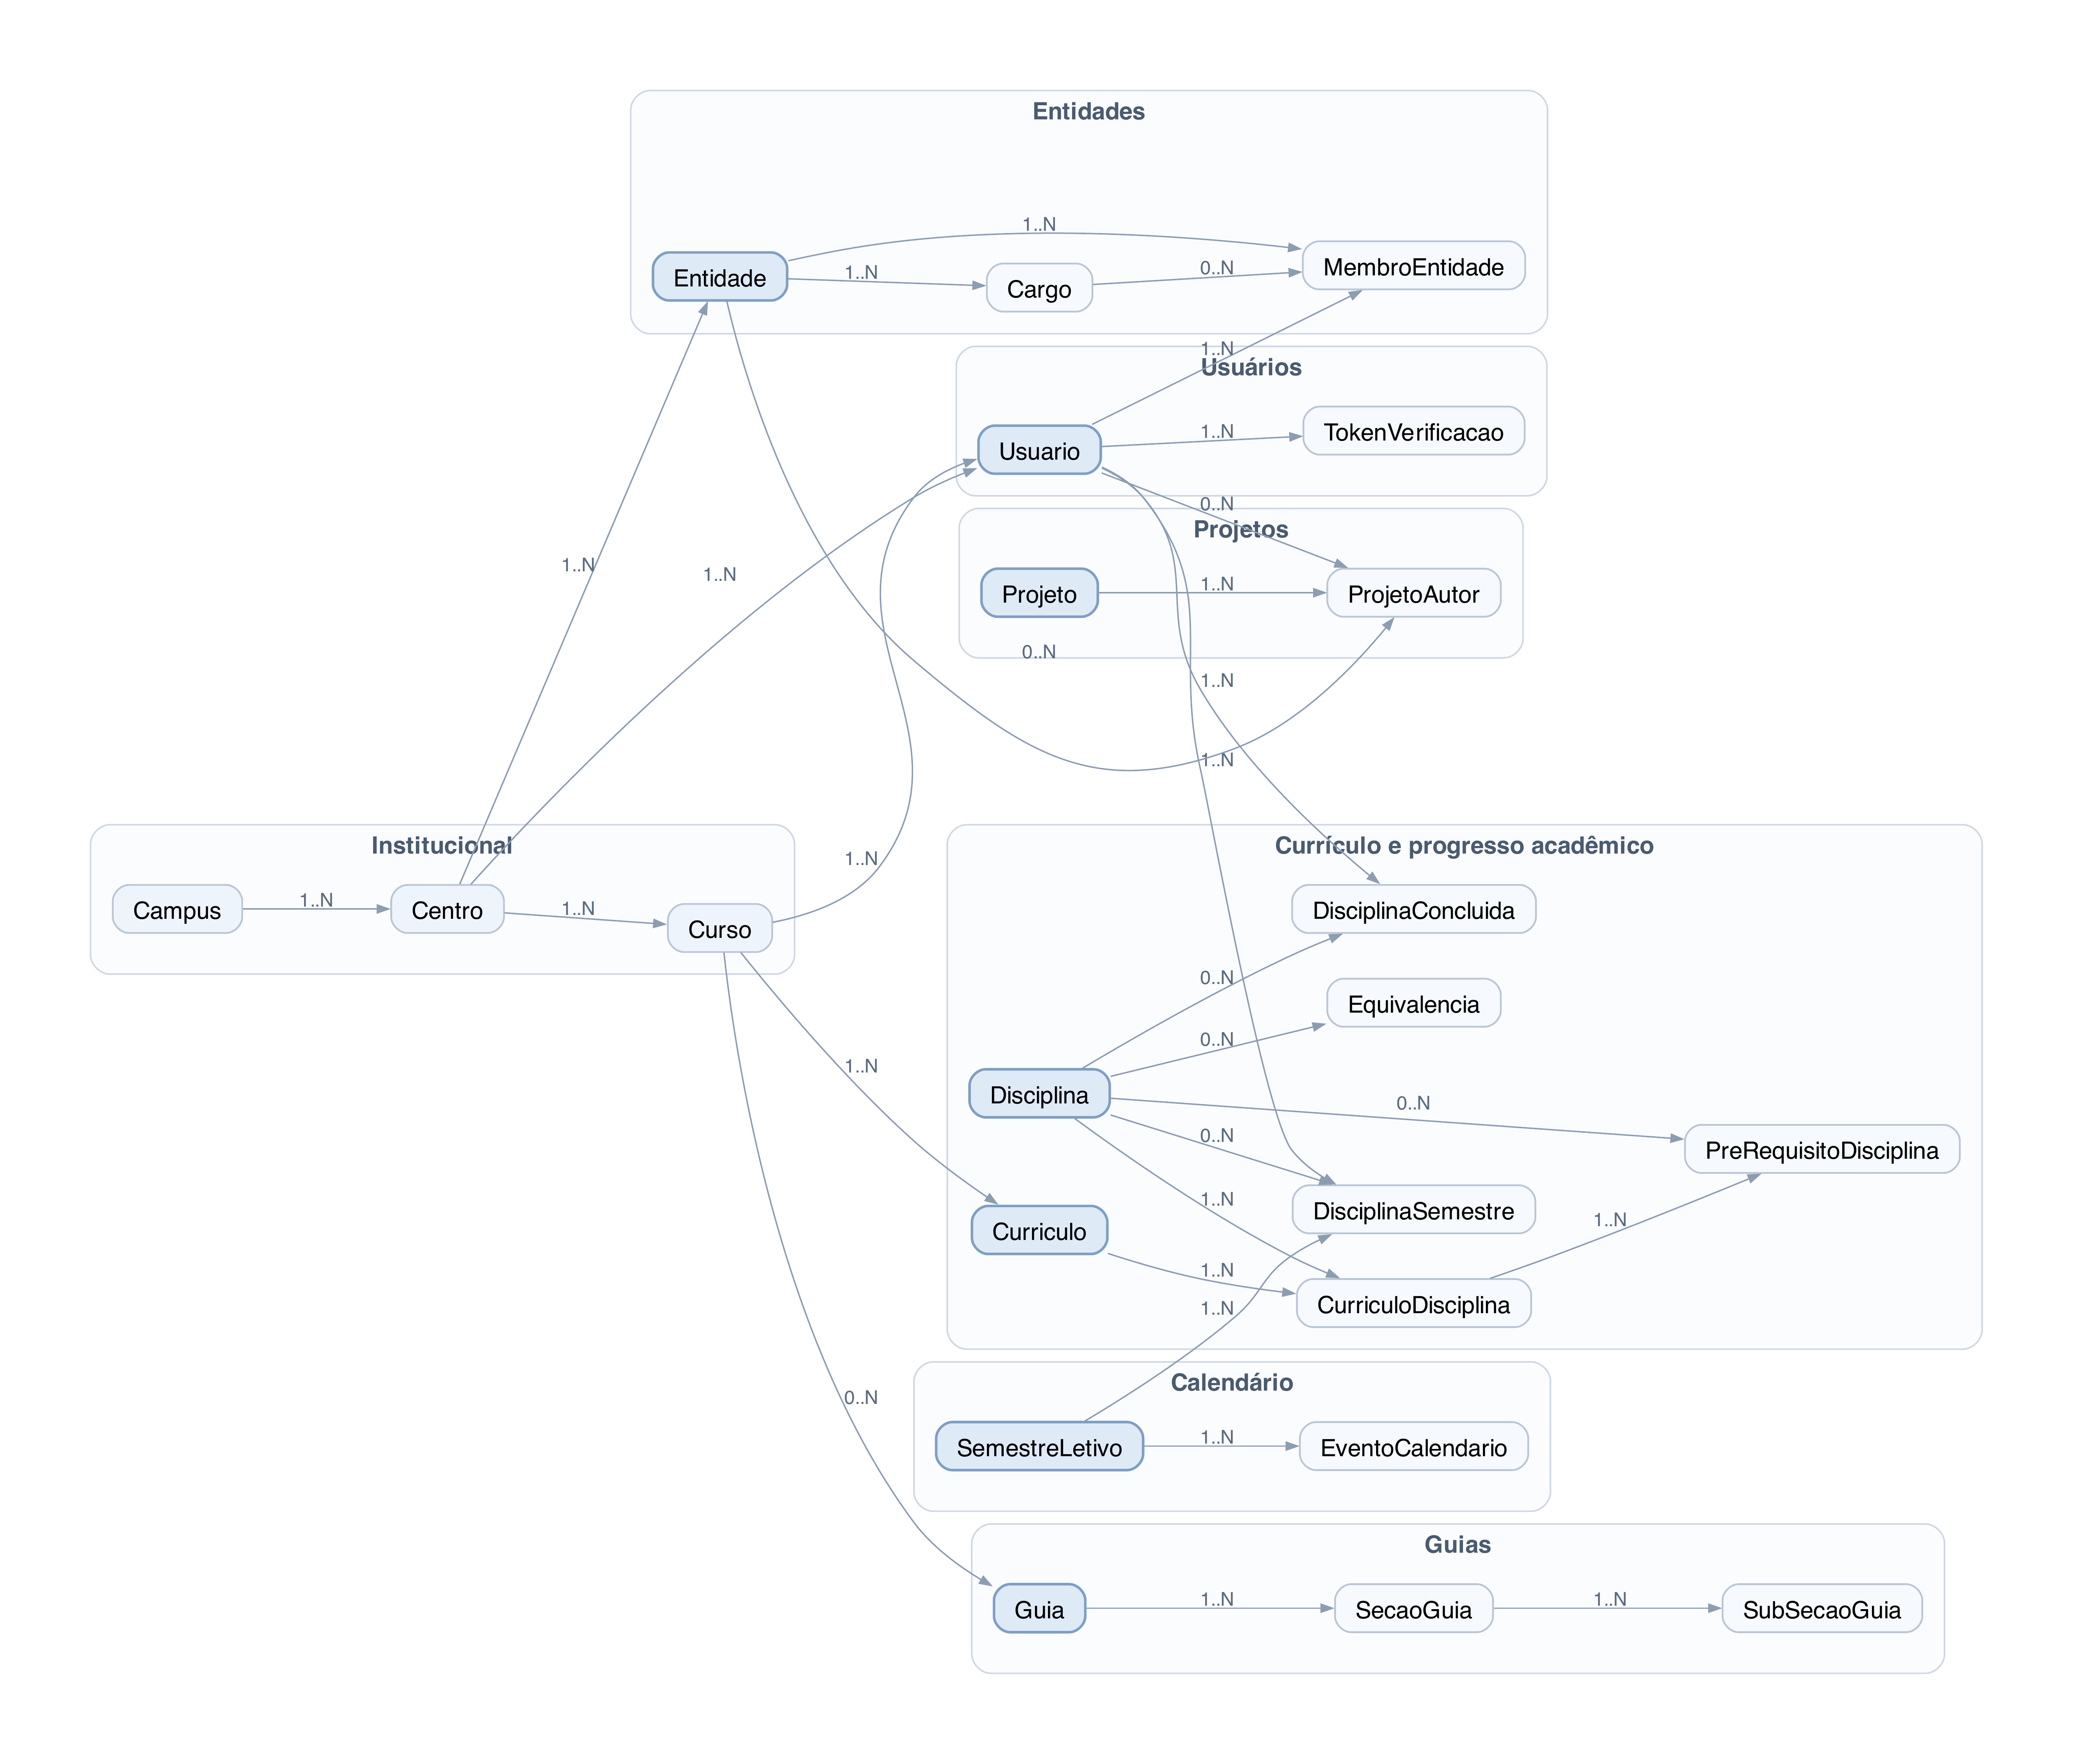
\includegraphics[height=0.78\textheight,keepaspectratio]{modelo-dados.pdf}\\[0.3em]
  \nota{Reserva \textperiodcentered{} Modelo de dados --- 23 modelos no schema}
\end{frame}

\end{document}
